\assignementTitle{Выбор участка территории}{35}{}

Для реализации проекта каждой команде необходимо определиться с участком территории для создания цифрового контента. Участок должен отвечать определенным техническим требованиям. Необходимо осуществить сбор и форматирование данных об объектах выбранного участка территории. Оформить собранные данные в виде файла формата json.

\textit{Подзадачи}
\begin{itemize} 
    \item Для выбранного сюжета квеста подберите участок города наиболее тематически подходящий. 
    \item Обоснуйте свой выбор в текстовой форме. От 2 - 5 предложений.
    \item Предоставьте выбранный участок в виде картинки.
    \item На выбранном участке города выбрать 10 мест-локаций, которые будут задействованы в игре
    \item На выбранный участок карты нужно нанести клеточные поля разных размеров.
    \item На клеточном поле отметить положение выбранных достопримечательностей. Выписать их координаты на поле (x,y) и их координаты в полярной системе(lat,long) ()
    \item Составить JSON по шаблону \url{https://drive.google.com/open?id=1jWv8mPx7t92utHmhF77srVI47jTJ_h7F}  в приложении
\end{itemize}

\markSection

\begin{enumerate}
    \item Наличие обоснования выбранной карты - \textit{5 баллов}.
    \item Отношение широты к высоте выбранного участка карты должно быть примерно равна золотому сечению. - \textit{3 балла}
    \item 3 клеточные карты - \textit{5,1 баллов}
    \item Есть координаты lat,long каждой достопримечательности - \textit{6,8 баллов}
    \item Есть координаты $x$, $y$ каждой достопримечательности - \textit{5,1 баллов}
    \item Координаты $x$, $y$ валидны. Т.е. координаты lat и lon: правильно переведены в правую систему координат для соответствующего клеточного поля, JSON по формату 1 составлен валидно - \textit{10 баллов}
\end{enumerate}

\solutionSection

\textit{Выбранный участок территории:}

\putImgWOCaption{10cm}{1}

На данном участке территории, в качестве точек интереса, определены 10 достопримечательностей, представленных в таблице.

\begin{tabular}{|p{8cm}|p{8cm}|}
    \hline
    \includegraphics[width=6.5cm]{2} & \includegraphics[width=8cm]{3} \\
    \hline
    Дом купца И.И. Базанова  (Гастроном №1)

    Карла Маркса, 25 
    
    52.284283, 104.287344
    
    Ранее: Дом купца И.И. Базанова & Дом Базанова (факультетские клиники ИГМУ) 

    Свердлова, 14 

    52.283765, 104.279034

    Ранее: Базановский воспитательный дом для детей до 1 года \\
    \hline
    \includegraphics[width=7cm]{4} & 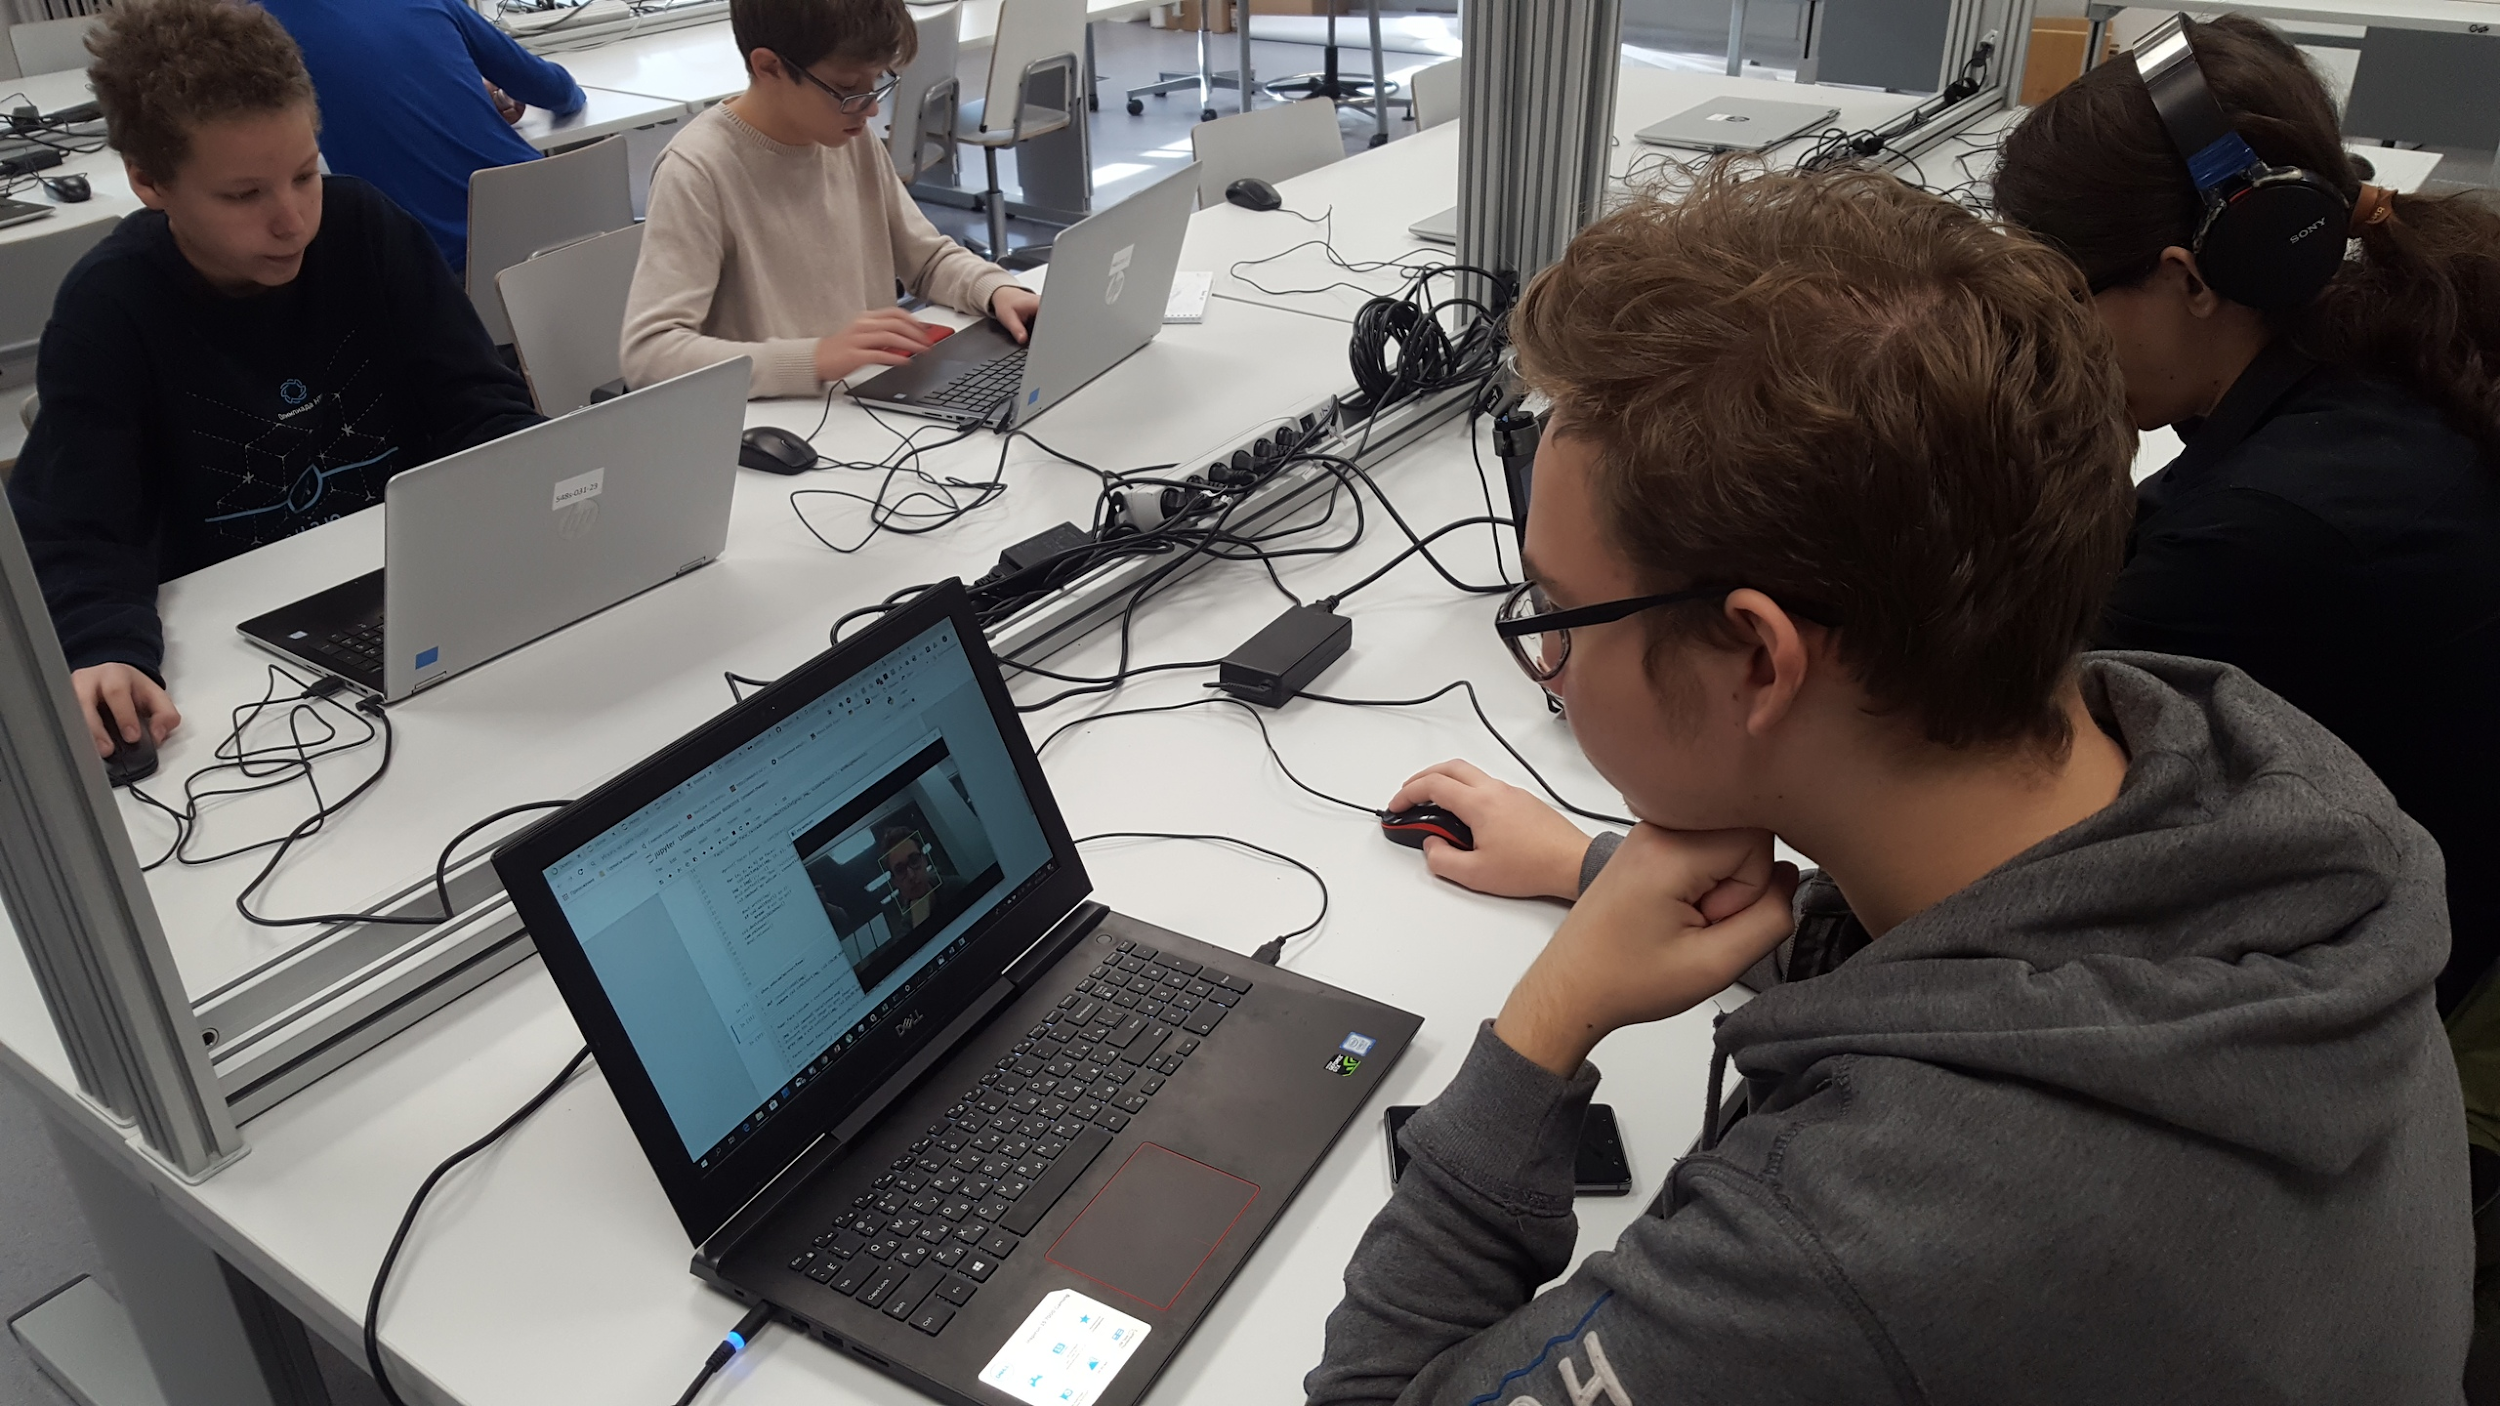
\includegraphics[width=6.5cm]{5} \\
    \hline
    Доходный дом Щербинина (Административное здание)

    Карла Маркса, 39 

    52.287527, 104.291251

    Ранее: Доходный дом с магазином Щербинина. & Усадьба Степанченкова 

    Дзержинского, 27 

    52.284905, 104.296066

    Ранее: Доходный дом  \\
    \hline
    \includegraphics[width=7cm]{6} & \includegraphics[width=7cm]{7} \\
    \hline
    Иркутская областная филармония 
    
    Дзержинского, 2 
    
    52.277985, 104.285367
    
    Ранее: ТРАМ (Театр рабочей молодежи) & Дом И.М. Файнберга  (отделы краеведения и библиографии, литературы по искусству и историко-культурного наследия областной библиотеки им. Молчанова-Сибирского)

    Халтурина, 1 

    52.289020, 104.286580

    Ранее: Доходный дом \\
    \hline
    \includegraphics[width=7cm]{8} & \includegraphics[width=7cm]{9} \\
    \hline
    Дворец детского и юношеского творчества 
    
    Желябова, 5 

    52.287770, 104.284846

    Ранее: особняк купца-миллионера А. Ф. Второва & Иркутский областной краеведческий музей 

    Карла Маркса, 13 
    
    52.281787, 104.284200 
    
    Ранее: сразу строился как Иркутский областной краеведческий музей \\
    \hline
    \includegraphics[width=7cm]{10} & \includegraphics[width=7cm]{11} \\
    \hline
    Иркутское театральное училище
    
    Тимирязева, 20
    
    52.280564, 104.295456 

    Ранее: Дом-усадьбу Абрама Элоевича Кринкевича & Городского начальное училище им. Н.В. Гоголя (МБОУ г. Иркутска СОШ №11)
    
    Богданова переулок, 6 

    52.286112, 104.284532
    
    Ранее: сразу строилось как Городского начальное училище им. Н.В. Гоголя \\
    \hline    
\end{tabular}

\subsubsection*{Обоснование:}

Проведение квеста на данном участке позволит участникам пройтись по самым интересным улицам города Иркутска. Здесь располагаются такие архитектурные сооружения как:  Доходный дом Щербинина, Дом купца И.И. Базанова, краеведческий музей, Усадьба Степанченкова. Эти и другие достопримечательности, которые задействованы в нашем квесте, как нельзя шире отображают характер города Иркутска. 


\markSection

Обоснование выбора карты есть и удовлетворяет поставленным условиям. Начисляется \textit{5 баллов.}

Ширина картинки равна 1513, а высота 995. Отношение широты к высоте тогда будет равно 1, 52, что примерно равно золотому сечению. Следовательно выбранный участок удовлетворяет условиям. Начисляется \textit{3 балла.}